\documentclass[12pt, conference]{IEEEtran}
% \IEEEoverridecommandlockouts
% The preceding line is only needed to identify funding in the first footnote. If that is unneeded, please comment it out.



\usepackage{cite}
\usepackage{amsmath,amssymb,amsfonts}
\usepackage{algorithmic}
\usepackage{graphicx}
\usepackage{textcomp}
\usepackage{xcolor}
\usepackage{hyperref}
\usepackage{wrapfig}
%for rotated figure
\usepackage{rotating}

\def\BibTeX{{\rm B\kern-.05em{\sc i\kern-.025em b}\kern-.08em
    T\kern-.1667em\lower.7ex\hbox{E}\kern-.125emX}}
    
% for image assets    
\graphicspath{ {./images/} }

\begin{document}

\title{A Software Solution for the Management and Distribution of Offline Class Recording Files}

\author{
\IEEEauthorblockN{George Paul}
\IEEEauthorblockA{\textit{IIIT, Hyderabad} \\
2021121006 \\
george.paul@research.iiit.ac.in}
}

\maketitle

\section{Abstract}
With the onset of of the COVID pandemic, many educational classes were held in online venues. These venues allowed for quick and easy recording of classes since it all went through online meetings/conference calls. The recordings were then usually hosted on the same websites.\\
As vaccines were developed and students returned to online classes, the issue of recordings became a problem as students had become used to them being available. This paper addresses the problem with an effective software solution.


\section{Related Work}
\subsection{MIT OpenCourseWare \cite{b1}}
The biggest and best example of a similar system in use is of MIT's OpenCourseWare. They demonstrate a class recording solution at a large scale and with a user base of the entire world.
The technology behind OCW is, by today's standards a little archaic. Even though the UI has been updated, the recording and video editing process remains manual. The video player used remains the same as it's always been and results in a lack of the bigger picture for students when they can't view what they want when they want to.
\subsection{YOLO \cite{b2}}
You Only Look Once is an approach to object that we use in this system to detect the instructor for the purposes of following them with the camera.\\
YOLO is the foremost method of object detection in the computer vision space right now besides the approach used with Region-based Convolutional Neural Networks.


\section{Problem Statement and Requirements}
The problem addressed in this paper is that of creating a software system to record, host and distribute recordings of offline classes among students of an institute. The system must be able to:
\subsection{Automatically Record}
Given video and audio input from cameras and microphones put up inside classrooms, the system must be able to extrapolate information as to the relevant information and viewpoints. The software must be able to track the instructors location and move camera views to maintain the instructors presence in the recordings.
\subsection{Observe Timings}
The software will automatically start and stop recordings of a class observing a certain early start and delay in stopping which can be specified by the administration.
\subsection{Upload and Hosting}
Once a class is over, the recording must soon, if not immediately, be available in the software's catalogue after the end of the class. The upload must be cautious of internet service interruptions and the recordings reliably.
\subsection{Hierarchical Access}
Students must, of course, be able to access the recordings for viewing purposes and be able to download any viewpoint they desire.\\
Teachers can login to the software to upload or delete recordings as they please. In addition to this they can also reorder recordings.
\subsection{Video Player}
The software will be equipped with a unique video player that is meant to show the view of the camera that is most relevant at that moment in the class, be it whether the board is being referred to or whether the instructor is speaking.


\section{System Design}
Every type of user is required to login and authenticate themselves with a username and password. The user is then presented with their respective frontend:
\subsection{Student User Stories}
\begin{itemize}
    \item{The main purpose of the student frontend is to show recordings. Students open the app to a list of recently recorded lectures and can also view the catalogue and can mark them as watched or not watched.}
    \item{The video viewer will feature 1-4 frames arranged as per the student's selected layout which can be changed at any time. The student can seek the videos to any point and have the recordings seek to the same point of time in all of the perspectives.}
    \item{The catalogue features the ability to sort by course and tag. The app will feature a comprehensive tag list from which videos can be tagged with up to 5 tags (limit can be changed from the admin dashboard). This helps the student to sort through recordings that are pertinent to a topic}
\end{itemize}
\subsection{Recorder User Stories}
The Recorder user is, in fact, completely automated. It has the ability to control the camera and microphone entirely. But despite that, it has access to many features which can be called upon by the Recorder Director script:
\begin{itemize}
    \item{The recorder can Start/Stop recording on a schedule described by a time table set by the Administrator. The recording will start $x$ minutes before the allotted time and will end $y$ minutes after. Both $x$ and $y$ can be set by the Administrator.}
    \item{The recorder can make calls to an API point that will allow it to send a frame of the recording to the server every $x$ seconds and receive data about adjustments needed to be made to the recording angle to better capture the instructor. The API point uses object detection algorithms to calculate a set of adjustments needed to be made according to the frame received.}
    \item{Once the recording is done, the recording will be uploaded to the backend via an API call.}
\end{itemize}
\subsection{Teacher User Stories}
\begin{itemize}
    \item{The teacher can add and remove recordings manually by entering a "Manage Recordings" page. The teacher can upload multiple perspectives as well.}
    \item{Tagging of recordings and ordering is done by the Teacher as well. Under the "Manage Recording" page, the Teacher can specify tags used for the course and use those tags to tag recordings.}
\end{itemize}
\subsection{Administrator}
\begin{itemize}
    \item{The administrator is in charge of allocating user accounts as either students, teachers or other administrators.}
    \item{Settings like the minutes before which to start, and after which to stop recording, are set by the administrator.}
\end{itemize}

\section*{Acknowledgments}
\begin{itemize}
    \item{\href{draw.io}{draw.io}, used to create the use case diagram}
\end{itemize}

\begin{thebibliography}{00}

\bibitem{b1} OpenCourseWare. Massachusetts Institute of Technology. \href{https://ocw.mit.edu/}{Home Page}
\bibitem{b2} Joseph Redmon, Santosh Divvala, Ross Girshick, Ali Farhadi. You Only Look Once: Unified, Real-Time Object Detection. \href{https://arxiv.org/abs/1506.02640v5}{arXiv:1506.02640}
\end{thebibliography}


\onecolumn

% \begin{figure}[h]
%     \centering
%     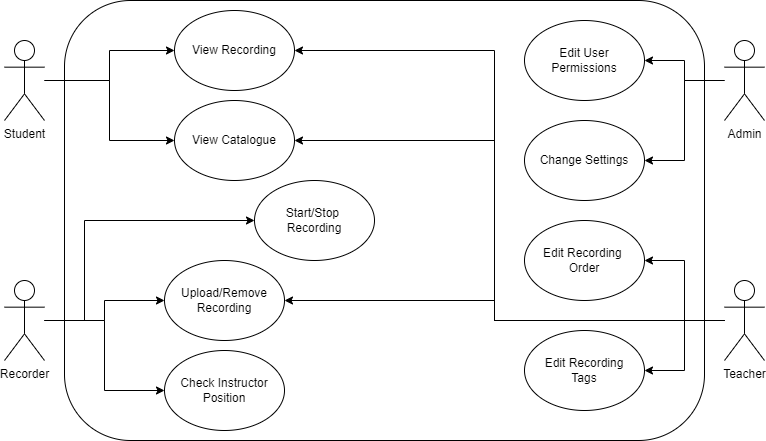
\includegraphics[width=10cm]{images/usecase.png}
%     \caption{Use Case diagram for the system}
% \end{figure}

\begin{sidewaysfigure}
    \centering
    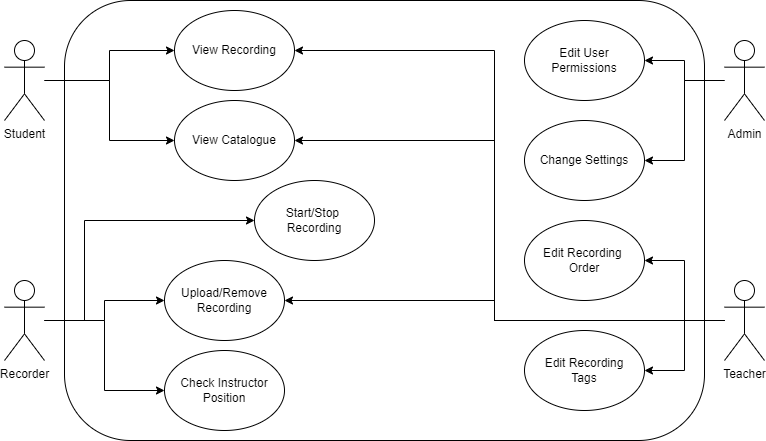
\includegraphics[width=22cm]{images/usecase.png}
    \caption{Use Case diagram for the system}
\end{sidewaysfigure}

\twocolumn

\end{document}